\documentclass[dissertation.tex]{subfiles}
\begin{document}

---------------------------------------------------------------

\begin{itemize}
  \item{
      Tishby produced a paper \cite{TISHBY} claiming to understand the basic
      principles of how DNNs work. 
    }
  \item{
      He decided to examine neural networks through the information domain,
      visualizing the results via Information Plane method \autoref{sec:IP}.
    }
  \item{
      Tishby made the claim that the incredible performance DNNs are able to
      achieve is due to the their ability to compress information inherent in
      the input data. Compressing data means the network is only able to keep
      relevant input features and it must forget the irrelevant bits of
      information, leading to the ability to generalize.
    }
  \item{
      Tishby made interesting claims and provided experimental evidence to
      support his claims, however he did not provide a formal proof leaving his
      results up for debate.
    }
  \item{
      Paper released by Saxe has contested the claims made by Tishby arguing
      that compression cannot happen in Neural Networks and the results are a
      consequence of the hyper parameters Tishby used.     
    }
  \item{
      However Saxes problem suffers from the same problem as Tishby's as it does
      not provide a formal proof only experimental evidence, as such it doesn't
      settle the rebuttal.
    }
  \item{
      To fully understand the discussion we need to understand the following
      topics Entropy and Mutual Information, Neural Networks, and Information
      Plane, described in \autoref{sec:EaMI}, \autoref{sec:NN}, and
      \autoref{sec:IP}.
    }
\end{itemize}

---------------------------------------------------------------

\section{Entropy and Mutual Information}
\label{sec:EaMI}

\textbf{Entropy} -- quantifies information content of a random variable. It is
generally measured in bits and can be though of as the expected information
content when we sample a random variable once. Let $X$ be a discrete random
variable that can take values in $\{x_1,...,x_n\}$. $H(X)$, the entropy of
$X$, is defined by \autoref{eq:entropy}.

\begin{equation}
  H(X)=-\sum _{i=1}^{n}{P (x_i)\log P(x_i)}
\label{eq:entropy}
\end{equation}

Consider a random variable $Y$ s.t $P(Y=1) = P(Y=0) = 0.5$, \autoref{eq:entropy}
defines $H(Y)$ to be 1.

Similarly for a random variable $Y$ s.t $P(Y=0) = 0.5, P(Y=1) = P(Y=2) = 0.25$,
we have $H(Y) = 1.5$.

\textbf{Conditional Entropy} -- quantifies the amount of information needed to
describe an outcome of variable $Y$ given that value of another random variable
$X$ is already known. Conditional Entropy of $Y$ given $X$ is written as
$H(Y|X)$. Let $X$ be defined as before, Let $Y$ be a discrete random variable
that can take values in $\{y_i,...,y_n\}$. The conditional entropy $H(Y|X)$ is
defined by \autoref{eq:condEntropy}.

\begin{equation}
H(Y|X)\ =-\sum _{x\in {X},y\in {Y}}P(x,y)\log {\frac {P(x,y)}{P(x)}}
\label{eq:condEntropy}
\end{equation}

Let the correlated variables $X$ and $Y$ be defined by \autoref{t:prob}.
\begin{table}[H]
  \centering
    \begin{tabular}{c|c|c}
      \diagbox{X}{Y} & 0 &1   \\
    \hline			
       0   &0.25&0.25 \\
    \hline			
       1   &0.5 &0 \\
  \end{tabular}
  \caption{Joint probability distribution for $X$ and $Y$}
  \label{t:prob}
\end{table}
\autoref{eq:entropy} and \autoref{eq:condEntropy} defines entropy values to be:
\begin{align}
  H(Y|X) &= 0.5 \nonumber \\
  H(X|Y) &\approx 0.6887 \nonumber \\
  H(X) &= 1 \nonumber \\
  H(Y) &\approx 0.8112 \label{eq:computedEntropies}
\end{align}

\textbf{Mutual Information (MI)} -- measures how much information two random
variables have in common. It quantifies information gained about one variable
when observing the other.  \autoref{eq:miExplicit} and \autoref{eq:miEntropy}
are two examples of how we can compute mutual information, using explicit
probability computations or entropies of the random variables respectively, here
$X$ and $Y$ are as previously defined.

\begin{equation}
      I(X,Y)=\sum _{y\in Y}\sum _{x\in X}{P(x,y)\log {\left({\frac
      {P(x,y)}{P(x)\,P(y)}}\right)}} 
\label{eq:miExplicit}
\end{equation}

\begin{equation}
  I(X, Y) = H(X) - H(X|Y)
\label{eq:miEntropy}
\end{equation}

For example of mutual information consider the random variables $X$ and $Y$ as
before in the conditional entropy section -- defined by \autoref{t:prob}. 

We computed the entropy values in \autoref{eq:computedEntropies}, we will use
them in \autoref{eq:miEntropy} to compute $I(X,Y)$.
\begin{equation}
  I(X,Y) = H(X) - H(X|Y) \approx 1 - 0.6887 = 0.3113
\end{equation}

\section{Neural Networks}
\label{sec:NN}

Before we understand neural networks we need to understand The Prediction
Problem and the purpose of Machine Learning Frameworks.

\subsection{The Prediction problem} 

Suppose we have some dataset $(x_i, y_i)$ for $i = 1,...,N$. The prediction
problem is finding a function $f$ s.t \autoref{eq:prediction} is satisfied.
\begin{equation}
  f(x_i) = y_i \text{ for } i = 1,...,N
  \label{eq:prediction}
\end{equation}
Prediction task is a common task that involves having input data
$\{x_i,...,x_N\}$ and finding the label, some desirable feature,
$\{y_i,...,y_N\}$. 

The prediction problem could be simple to extract: for example if our input is a
natural number $x_i\in\mathbb{N}$, and our label is either $true$ or $false$
depending if $x$ is even or odd -- in which case function defined by
\autoref{eq:evenodd} satisfies the problem.  \begin{equation}
  g(x) = \begin{cases}
    True, & \text{if } \exists n\in\mathbb{N}.x = 2n , \\
    False, & \text{otherwise}.
  \end{cases}
\label{eq:evenodd}
\end{equation}
The prediction problem also can be impossible to solve: for example the halting
problem, if our $x`s$ are programs and $y`s$ boolean values corresponding if the
program halts or not.


Of course the prediction problem can be hard or impossible to solve as is the
case for problems:
\begin{table}[H]
  \centering
    \begin{tabular}{l|l|l}
      input data & label & difficulty \\ 
      \hline
      \rowcolor{Gray}
      medical symptoms & diagnosis & intractable \\ 
      picture  & object in the picture &  \\ 
      \rowcolor{Gray}
      face photograph  & identity &  \\ 
      stock market history  & future stock prices &  \\ 
      \rowcolor{Gray}
      program  & does the program halt & proved to be unsolvable \\ 
      boolean equation  & is the equation satisfiable & expensive to compute 
  \end{tabular}
  \caption{Example of specific prediction problems }
  \label{t:prediction}
\end{table}

Problems listed in \autoref{t:prediction} are either intractable, unsolvable or
too expensive to compute -- hence we cannot produce an algorithm that always
give the correct answer and runs in a reasonable time.

\subsection{Machine Learning Frameworks}

If the Prediction problem is too difficult and we are tolerant to errors in our
labels we may want to use a supervised machine learning framework\footnote{In
this thesis we are exclusively talking about supervised machine learning
techniques -- the word "supervised" will be omitted for brevity} to tackle the
problem. 

Every machine learning framework requires that we have some subset
$\hat{X}\subseteq\{x_i,...,x_N\}$ s.t that $ \forall x\in\hat{X}$ we know label
the $y$. A framework uses the data in order to reach some goal -- such as
minimizing the prediction error. The way any machine learning framework learns
from data varies, but generally more data means an increase in prediction
performance.

\subsection{Neural Networks} 

Neural Networks (\textbf{NN}) are an example of a machine learning framework. They learn
from data and attempt to solve the prediction problem.

The structure of a NN consists of layers of nodes, where every consecutive
layer is fully connected as in \autoref{fig:nnOriginal}.  When we try to
predict a label of a specific input every node gets assigned a value in the
real number space $\mathbb{R}$. Values for the Input nodes are provided,
whereas values for the nodes in non-input layers are generated based on nodes
from the preceding layer. Let $n_{l,i}$ be the value that the $i'th$ node in
layer $l$ takes. Let $w_{l,j,i}$ be a parameter that influences how relevant
the $j'th$ node in layer $l$ is to the $i'th$ node in layer $l+1$.
\begin{equation}
  n_{l+1,i} = f(\sum_{j = 0}^{\text{layer }l\text{ size}} w_{l,j,i}*n_{l,j})
  \label{eq:nextNode}
\end{equation}
$f$ in \autoref{eq:nextNode} is called the activation function and is generally 
taken to be:
\begin{itemize}
  \item{
      ReLu: $f(x) = max(0, x)$
    }
  \item{
      Sigmoid: $f(x) = \frac{1}{1+e^x}$
    }
  \item{
      Tanh: $f(x) = tanh(x)$
    }
\end{itemize}

For our purposes we will extract away the individual nodes in the network and
only consider the layers -- as in \autoref{fig:nnModified}.
\begin{figure}[H]
  \centering
  \begin{subfigure}[t]{0.49\textwidth}
    \centering
    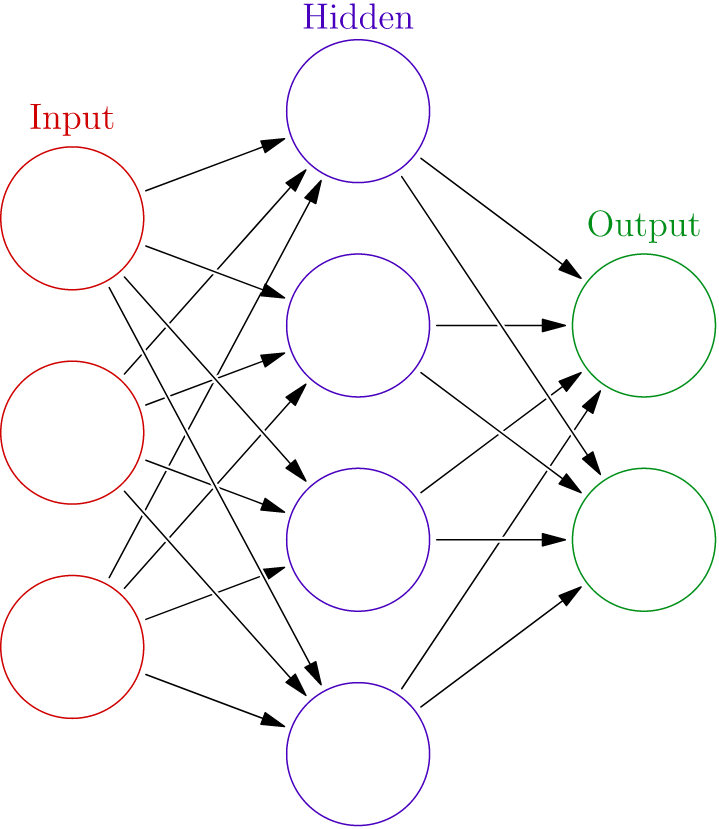
\includegraphics[width=0.6\textwidth]{figs/neural_network.png}
    \caption{
      Structure of a typical neural network.
    }
    \label{fig:nnOriginal}
  \end{subfigure}
  \hfill
  \begin{subfigure}[t]{0.49\textwidth}
    \centering
    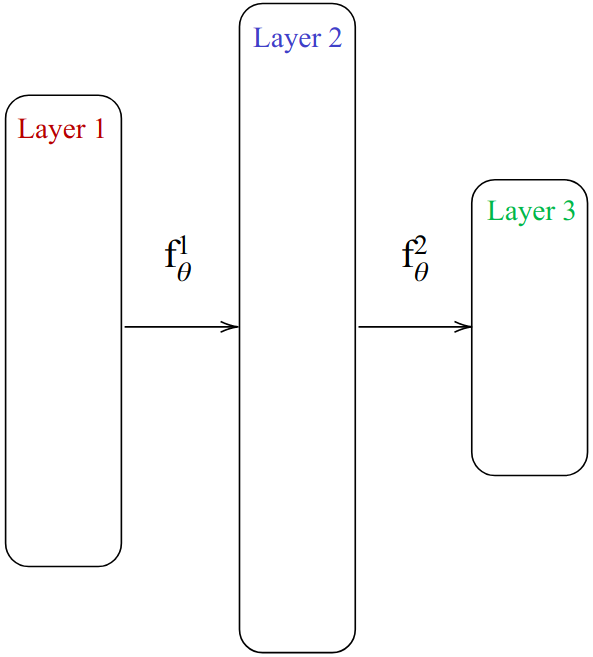
\includegraphics[width=0.6\textwidth]{figs/neural_network_abstraction.png}
    \caption{
      Structure of our abstracted neural network.
    }
    \label{fig:nnModified}
  \end{subfigure}
    \caption{
      Source: Wikimedia Commons 
    }
\end{figure}

We will formally define a neural network to be a sequence of functions
$f_{\theta}^1,f_{\theta}^2,...,f_{\theta}^L$ that are parameterized by
$\theta$ s.t. Equations \ref{eq:nnTransitions}.

\vbox{
\begin{align}
	\text{let } t_0 &= x, \nonumber \\
  t_0 \rightarrow f_{\theta}^1(t_0) &= t_1, \nonumber \\
  t_1 \rightarrow f_{\theta}^2(t_1) &= t_2, \nonumber \\
  &... \nonumber \\
  t_{N-1} \rightarrow f_{\theta}^N(t_{N-1}) &= t_N, \nonumber\\
  \text{let } \hat{y} &= t_N
\end{align}
\vspace*{-\baselineskip}
\vspace*{-\baselineskip}
\begin{gather}
  \text{values } t_1,t_2,...,t_N 
  \text{ here are } \textbf{activations } \text{of layers } 1,2,...,N,
	\nonumber\\
	x \text{ is any input to the NN from the set } \{x_i,...,x_N\}, \nonumber\\
	\hat{y} \text{ is the prediction of the NN for the input,} x
	\text{ which may or not be correct label,} \nonumber\\
	\rightarrow\text{ signifies a transition from one NN layer to another.}
	\nonumber
\end{gather}
}


------------------------------------------------------------------

Neural Networks are a machine learning framework, they have been used
effectively in predicting and classifying data.

Suppose we have a dataset:
\begin{align*}
  &(x_i, y_i) \text{ for } i = 1,...,N \\
  &\text{where, } x_i \in \mathbb{R}^d, y_i \in \mathbb{R}^{d^\prime}
\end{align*}
where $x_i$ is the input to the Neural Network and $y_i$ is the label or the
value we want the neural network to predict. For example suppose we are trying
to classify if an image contains a cat or no, then $x_i$ would be an encoding of
an image and the label $y_i$ could be 1 if the image contains a cat and 0 if it
does not.

The network is structured in layers where every layer holds an intermediate
representation of the final prediction output -- let us call this intermediate
representation an \textbf{activation} of that specific layer. For our purposes
we will define a neural network to be a sequence of functions
$f_{\theta}^1,f_{\theta}^2,...,f_{\theta}^L$ that are parameterized by weights
$\theta$ s.t

\vbox{
\begin{center}
\end{center}



\tikzset{every picture/.style={line width=0.75pt}} %set default line width to 0.75pt        

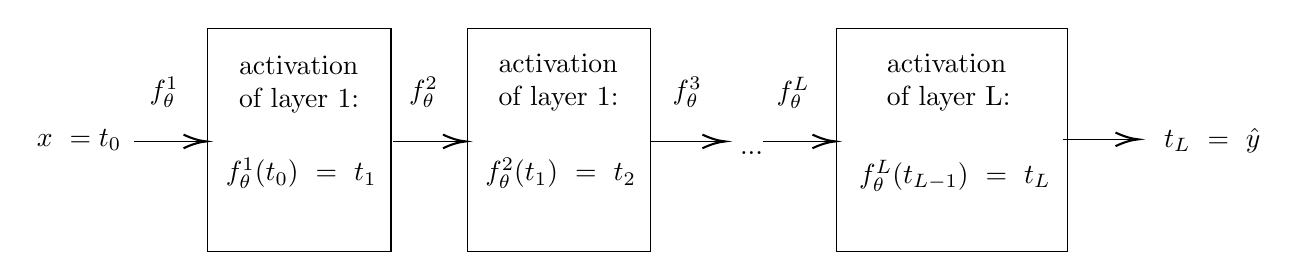
\begin{tikzpicture}[x=0.75pt,y=0.75pt,yscale=-1,xscale=1]
%uncomment if require: \path (0,244.52349853515625); %set diagram left start at 0, and has height of 244.52349853515625

%Shape: Rectangle [id:dp11557839760136379] 
\draw   (86,115) -- (174.28,115) -- (174.28,222.54) -- (86,222.54) -- cycle ;
%Straight Lines [id:da1142035093360374] 
\draw    (50.28,169.54) -- (83.28,169.54) ;
\draw [shift={(85.28,169.54)}, rotate = 180] [color={rgb, 255:red, 0; green, 0; blue, 0 }  ][line width=0.75]    (10.93,-3.29) .. controls (6.95,-1.4) and (3.31,-0.3) .. (0,0) .. controls (3.31,0.3) and (6.95,1.4) .. (10.93,3.29)   ;

%Straight Lines [id:da3402708303870947] 
\draw    (299.28,169.54) -- (333.28,169.54) ;
\draw [shift={(335.28,169.54)}, rotate = 180] [color={rgb, 255:red, 0; green, 0; blue, 0 }  ][line width=0.75]    (10.93,-3.29) .. controls (6.95,-1.4) and (3.31,-0.3) .. (0,0) .. controls (3.31,0.3) and (6.95,1.4) .. (10.93,3.29)   ;

%Straight Lines [id:da9984222042248518] 
\draw    (498.28,168.54) -- (532.28,168.54) ;
\draw [shift={(534.28,168.54)}, rotate = 180] [color={rgb, 255:red, 0; green, 0; blue, 0 }  ][line width=0.75]    (10.93,-3.29) .. controls (6.95,-1.4) and (3.31,-0.3) .. (0,0) .. controls (3.31,0.3) and (6.95,1.4) .. (10.93,3.29)   ;

%Shape: Rectangle [id:dp7529094555455995] 
\draw   (211,115) -- (299.28,115) -- (299.28,222.54) -- (211,222.54) -- cycle ;
%Straight Lines [id:da3983438928921348] 
\draw    (175.28,169.54) -- (208.28,169.54) ;
\draw [shift={(210.28,169.54)}, rotate = 180] [color={rgb, 255:red, 0; green, 0; blue, 0 }  ][line width=0.75]    (10.93,-3.29) .. controls (6.95,-1.4) and (3.31,-0.3) .. (0,0) .. controls (3.31,0.3) and (6.95,1.4) .. (10.93,3.29)   ;

%Shape: Rectangle [id:dp3082851546438703] 
\draw   (389,115) -- (500.28,115) -- (500.28,222.54) -- (389,222.54) -- cycle ;
%Straight Lines [id:da29571517496636934] 
\draw    (353.28,169.54) -- (386.28,169.54) ;
\draw [shift={(388.28,169.54)}, rotate = 180] [color={rgb, 255:red, 0; green, 0; blue, 0 }  ][line width=0.75]    (10.93,-3.29) .. controls (6.95,-1.4) and (3.31,-0.3) .. (0,0) .. controls (3.31,0.3) and (6.95,1.4) .. (10.93,3.29)   ;


% Text Node
\draw (65,146) node   {$f^{1}_{\theta }$};
% Text Node
\draw (130,142) node  [align=left] {activation \\of layer 1: };
% Text Node
\draw (131,185) node   {$f^{1}_{\theta }( t_{0}) \ =\ t_{1}$};
% Text Node
\draw (24,169) node   {$x\ =t_{0}$};
% Text Node
\draw (348,175) node   {$...$};
% Text Node
\draw (317,146) node   {$f^{3}_{\theta }$};
% Text Node
\draw (570,169) node   {$t_{L} \ =\ \hat{y}$};
% Text Node
\draw (190,146) node   {$f^{2}_{\theta }$};
% Text Node
\draw (255,141) node  [align=left] {activation \\of layer 1: };
% Text Node
\draw (256,185) node   {$f^{2}_{\theta }( t_{1}) \ =\ t_{2}$};
% Text Node
\draw (368,146) node   {$f^{L}_{\theta }$};
% Text Node
\draw (443,141) node  [align=left] {activation \\of layer L: };
% Text Node
\draw (446,186) node   {$f^{L}_{\theta }( t_{L-1}) \ =\ t_{L}$};


\end{tikzpicture}
\begin{center}



\end{center}

\vspace*{-\baselineskip}
\vspace*{-\baselineskip}
\begin{figure}[H]
  \centering
  \caption{
    Visualization of a neural networks structure.  $x$ here is any input to the
    network from the set $\{x_i,...,x_N\}$.  $\hat{y}$ is the prediction of the
    network for the input $x$ which may or may not be to the correct label. The
    values $t_1,...,t_L$ here are \textbf{activations} of layers $1,...,L$.
  }
  \label{fig:network}
\end{figure}
}

We have one function for each layer transition of the neural network this allows
us to extract the activation of a specific layer as in \autoref{eq:layerL} -- we
will need to get access to intermediate layers in our experiments.

\begin{figure}[H]
  \[ t_l = f_{\theta}^l(f_{\theta}^{l-1}(...(f_{\theta}^1(x)))) \]
  \caption{\textbf{activation} of layer l for input x}
  \label{eq:layerL}
\end{figure}

\textbf{Stochastic Gradient Descent} Each of the transition function are
parameterized by the weights function $\theta$. The $\theta$ function is
directly controlled by Stochastic Gradient Descent (SGD) algorithm.  SGD is an
algorithm for training a neural network it gradually updates the weights
$\theta$ according to some goal such as minimising the prediction error.  SGD is
an iterative process, it has a notion of epochs where one iteration of the
algorithm advances epochs by one, this implies that $\theta$ function depends on
which epoch we are currently at thus it must take the epoch number as an
argument -- $\theta(e)$.

\section{The Information plane}
\label{sec:IP}

\subsection{Setup}

The Information plane is a way of visualizing the Neural Network`s training
process through the information domain. By looking at mutual information between
the input $X$ the intermediate neural network layer activations $T$ and the
label $Y$ we can see how the information flows through the network.

Mutual Information is only applicable to Probability distributions, however we
only have the dataset $(x_i, y_i) \text{ for } i = 1...N$ , if we assume that
every input $x_i$ equally likely we can provide a routine that defines our
probability distribution.

For convenience let us define $F_{\theta}^t$ to be the activation of layer t given
input $x$, i.e
\begin{equation}
  F_{\theta}^t(x) = f_{\theta}^t(f_{\theta}^{t-1}(...(f_{\theta}^1(x))))
  \label{eq:bigF}
\end{equation}


Consider \autoref{fig:rxty}, the routine defines the random variables
$X,T_{e,t},Y$. Here $T_{e,t}$ is the distribution of layer $t$ for the epoch $e$,
$X$ and $Y$ is the original data with assumption that it is uniformly
distributed. 

Using the probability distributions we now have values:
\begin{itemize}
  \item{
      $I(T_{e,t}, X)$ -- Mutual Information between the input distribution and the
      layer activations 
    }
  \item{
      $I(T_{e,t}, Y)$ -- Mutual Information between the label distribution and the
      layer activations.
    }
\end{itemize}
This allows us to generate the Information plane.


\begin{figure}[H]
    \begin{pythonfigure}
      def rxty(e, t):
        pick i ;$\sim$; Uniform {1...N}
        return ;$(x_i, F_{\theta(e)}^t(x_i), y_i)$;
    \end{pythonfigure}
    \caption{Definition of correlated random variables $X, T_{e,t}$ and, $Y$}
    \label{fig:rxty}
\end{figure}

\subsection{Visualization}

The Information plane visualizes the whole training process, in order to
generate the information plane we need $I(X,T_{e,t})$ and $I(Y,T_{e,t})$ for every
epoch $e$ and every layer $t$.

Consider for now that we only trained our neural network for one epoch, the
\autoref{fig:Ip1} shows an example of this. 

In this case the network consists of 5 layers, in the figure every node
corresponds to a distinct layer. The lines between the nodes help us distinguish
epochs from each other and gives helps us to see the order of the layers, the
upper-right-most node corresponds to the first layer in the neural network, the
lower-left-most node corresponds to the fifth and last layer of the network.

Consider now \autoref{fig:Ip2}, it shows an information plane for a full
training phase. The color signifies what epoch the data belongs to and lets us
see how the network progressed over time. We can see that at the start $I(Y,
T_{1,4}) \approx 0$ meaning the network has not preserved any information about
the label distribution $Y$, but by the end of the training we see $I(Y,
T_{10^4,4}) \approx 1$ which means we have preserved almost all the information
about the label.

\begin{figure}[H]
  \centering
  \begin{subfigure}[t]{0.48\textwidth}
    \centering
    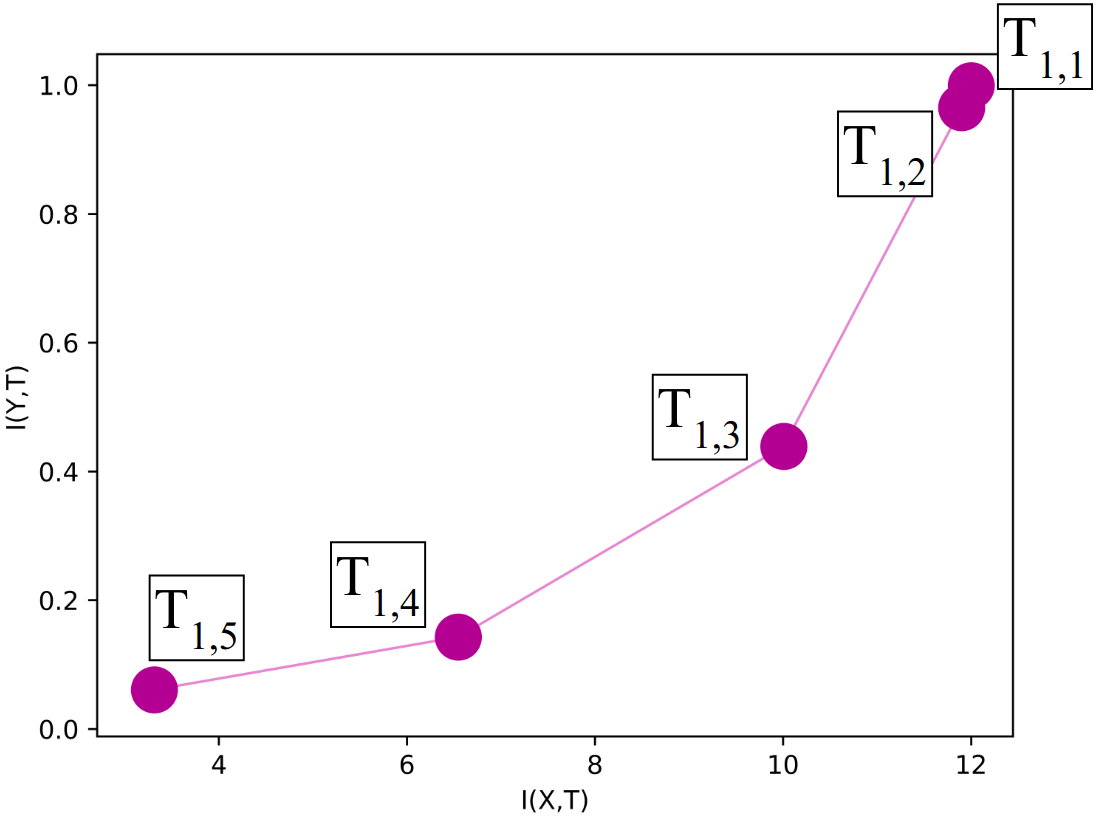
\includegraphics[width=\textwidth]{figs/ip_1v3.png}
    \caption{
      information plane for a neural network with 5 layers, which was only trained
      for one epoch.
    }
    \label{fig:Ip1}
  \end{subfigure}
  \hfill
  \begin{subfigure}[t]{0.5\textwidth}
    \centering
    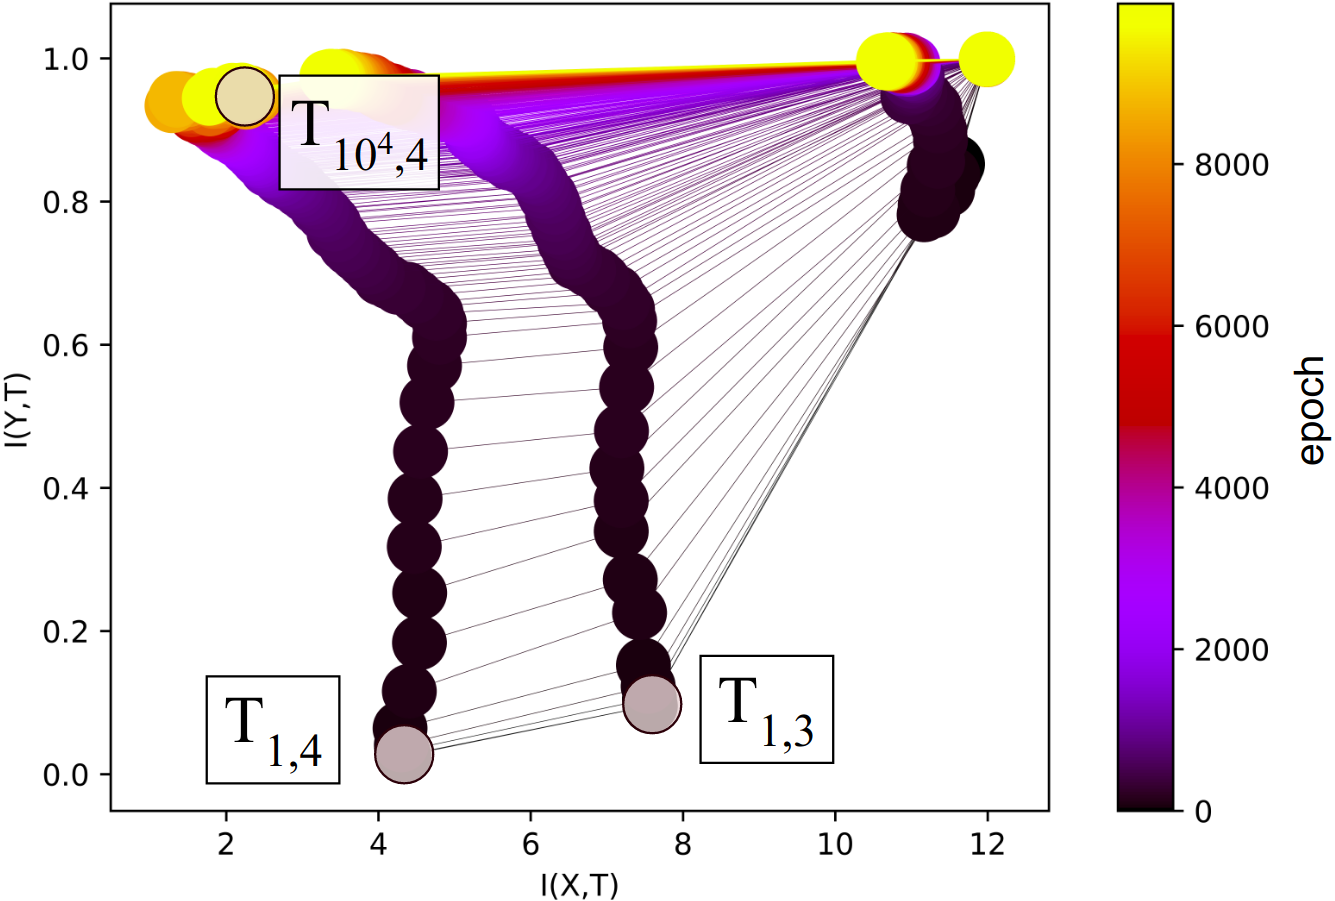
\includegraphics[width=\textwidth]{figs/ip_10000v3.png}
    \caption{
      Information plane for a neural network with 4 layers, which was trained
      for approximately $10\,000$ epochs.
    }
    \label{fig:Ip2}
  \end{subfigure}
  \caption{
    The Neural Networks in both figures have been trained on the same dataset as
    used by Tishby\cite{TISHBY}, hence input entropy, $H(X)$, is 12 and
    label entropy, $H(Y)$, is 1.
    Some Nodes are labeled $T_{e,l}$, where $e$ is the epoch number and $l$ is
    the layer the node belongs to. Consider $T_{1,3}$ from Figure (b) -- The
    node corresponds to the information content of layer 3 for the 1'st epoch,
    the $x$ coordinate of the node is the value $I(X, T_{1,3})\approx{8}$, the
    $y$ coordinate is the value $I(Y, T_{1,3})\approx{0.1}$
  }
\end{figure}

\subsection{Interpretation of the Information Plane}

Let us once again consider \autoref{fig:Ip2}, we can see two phases in the figure
Tishby has named them The Fitting Phase and The Compression Phase.

\subparagraph{The Fitting Phase} In \autoref{fig:Ip2} the neural network is in
the fitting phase from the start of the training up until epoch $\sim$1500. The
duration of the fitting phase varies heavily on the training parameters and is
most influenced by the size of our input dataset. The fitting phase is
characterized by:
\begin{itemize}
  \item{
      A rapid increase in $I(Y, T_{e,t})$, the information about the label, as we
      advance through the epochs $e$, the increase is especially visible in the
      later layers, in our case layers 3 and 4.
    }
  \item{
      Either an increase or no change in $I(X, T_{e,t})$, the information about
      the input, as we advance through the epochs $e$, in our case we see very
      little change in $I(X,T_{e,t})$.
    }
\end{itemize}

During the fitting phase a neural network tries to memorize the data and make
predictions based on the observations, this means that the network may learn
useless features that only superficially correlate with the correct label.

\subparagraph{The Compression Phase} In \autoref{fig:Ip2} the neural network
enters the compression phase when the fitting phase ends around epoch $\sim$1500
and lasts until we finish the training process. The compression phase is
characterized by:
\begin{itemize}
  \item{
      A slowdown of how fast $I(Y, T_{e,t})$ is increasing with respect to epochs
      $e$. 
    }
  \item{
      A slow decrease of $I(X, T_{e,t})$ with respect to epoch $e$.
    }
\end{itemize}

During the compression phase a neural network compresses representation of the
input discarding more features that did not help with predicting correct labels.
Discarding irrelevant features helps the neural network generalize and produce
better predictions for new data. 


---------------------------------------------------------------


Before developing a plan for how we are going to realize the project in code we
needed to fully understand the ideas presented in the paper:
\begin{itemize}
    \begin{item}
      We needed to identify the main ideas of the paper and understand why some
      parts of the paper are not agreed upon in the scientific community.
      Understand why his ideas are contentious and whether reproducing his
      experiments could bring more validity to his claims. This involved reading
      papers published by Tishby and academics who shown an opposing view to
      him.
    \end{item}
    \begin{item}
      A main tool that the paper relies on is MIE (Mutual Information
      Estimation). Reading about MIE we quickly understood that MIE is a
      contentious part of the project as a result we had to do a decent amount
      of research regarding the subject. MIE is difficult because we are trying
      to estimate information between two continuous distributions using only a
      discrete sample set. This area has not seen much academic attention so the
      tools we ended up using could be greatly improved in the future.
    \end{item}
\end{itemize}

Once we had a reasonable understanding of the ideas in the paper and which areas
needed more attention we diverted our attention to figuring out the details of
how the experiments were conducted figure out what hyper parameters Tishby
decided are important and what assumptions he made whilst devising the
experiments. 

In addition we needed to find out what resources are available to us online,
what programming frameworks we are going to use for the projects implementation,
and to think about possible extensions to the project once the success criteria
has been achieved.

\begin{itemize}
  \item{
      Online Resources: The two main papers by Tishby and by Saxe have made
      their code public online via Github, we made 

      Online Resources: The two main papers we were looking at has made their
      code available to the public via Github, the papers are Tishby`s paper and
      the main opposing paper by Saxe.
    }
  \item{
      Programming frameworks: The original experiment implementation by Tishby
      has used the Tensorflow framework. We have decided to use the Keras
      framework as it produces code that is more concise and is easier to
      read/maintain. Furthermore rewriting the experiments in a different
      framework means that we cannot rely on the details of Tishby's and
      potentially avoid any mistakes that may exist in the original
      implementation.
    }
    \begin{item}

      Thinking about how we could extend the project helped us understand the
      scope of the project and what areas were most important and/or interesting
      to us. 

      We came up with a couple of extensions before having written any code but
      the most interesting one only materialized after a good deal amount of
      work into the project (that is the AS-IF-Random experiment described
      below)

      \begin{itemize}
        \item{
            Different Datasets : the most straight forward extension to the
            project just using different dataset to the one Tishby used. This is
            essentially just varying one of the parameters in the Neural
            Network. (Implemented)
          }
        \item{
            Quantized Neural Network : the idea behind this was to only allow
            single neurons to acquire values in a given range say 1...256. This
            would make the distribution within a DNN later discrete and hence it
            would make calculating mutual information straightforward. (Not
            Implemented)
          }
        \item{
            As-If-Random : one problem with Tishby's work is that he calculates
            mutual information for a single epoch at a time which by definition
            is zero (in his paper he tries to justify the result will explore
            this later) this extension tries to explore the weights of a neural
            network as random variables by calculating mutual information for
            multiple epochs at a time.
          }
      \end{itemize}
    \end{item}
\end{itemize}

\end{document}
